\documentclass[10pt,a4paper,openany,twoside]{book}

\usepackage{layout_cours}
\usepackage{hyperref}
\usepackage{colortbl}

\setlist{leftmargin=5mm}

\begin{document}
	\chapnumber{2} % numéro du chapitre
	\titre{Probabilités conditionnelles} % titre du chapitre
	\classe{Terminale STMG} % classe
	\entetegal

\section{Vocabulaire probabiliste}

\begin{defi}{Issue, univers}{}
   Chaque résultat possible d'une \textbf{expérience aléatoire} est appelé \textbf{issue}.

   L'ensemble formé par les issues est appelé \textbf{univers}, il est souvent noté $\Omega$.
\end{defi}

\begin{ex}{}{}
   $5$ est une issue dans le cas d'un lancer de dé à six faces : $\Omega =\{~1~;~2~;~3~;~4~;~5~;~6~\}$.
\end{ex}

\begin{defi}{Evénement}{}
   Un \textbf{événement} de l'expérience aléatoire est une partie de l'univers. Il est composé d'une ou plusieurs issues.
\end{defi}

\begin{ex}{}{}
   $B$ : \og obtenir un numéro pair \fg{} est un événement correspondant à $B=\{~2~;~4~;~6~\}$.
\end{ex}

\begin{defi}{Evénement contraire}{}
   Pour tout événement $A$ il existe un événement noté $\overline{A}$ et appelé \textbf{événement contraire} de $A$, qui est composé des éléments de $\Omega$ qui ne sont pas dans A.
\end{defi}

\begin{ex}{}{lancer_de}
   On considère un lancer de dé à six faces. Soit $A$:\og obtenir un nombre inférieur à $4$ \fg{}. Alors son événement contraire est $\overline{A}$:\og obtenir $5$ ou $6$ \fg{}.
\end{ex}

\begin{defi}{Probabilité d'un événement}{}
   La \textbf{probabilité d'un événement} $A$ est un nombre entre $0$ et $1$ noté $\P(A)$ qui indique si cet événement se réalise souvent lorsqu'on répète l'expérience.
\end{defi}

\begin{ex}{}{}
   Avec l'exemple \ref{exe:lancer_de}, on a $\P(A)=\frac{4}{6}=0.66\dots$, car on est dans une situation \textbf{d'équiprobabilité}. Chaque numéro sur le dé a la même probabilité (à savoir une chance sur six).

   $\P(\overline{A})=1-\P(A) = \frac{2}{6}$. Il y a deux chances sur six d'obtenir le contraire de $A$, à savoir obtenir un nombre supérieur strictement à 4.
\end{ex}

\section{Intersection et réunion d'événements}

\begin{defi}{Intersection et réunion}{}
\begin{minipage}{9cm}
\textbf{Intersection d'événements} : l'événement constitué des issues appartenant à $A$ et à $B$ est noté $A\cap B$

\end{minipage}
\begin{minipage}{5cm}
\begin{center}
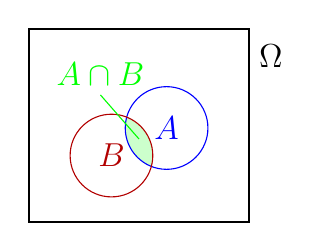
\begin{tikzpicture}[scale=0.7]
\draw[color=black,thick] (-2cm, -1.5cm) rectangle (2cm, 2cm);
\node[color=black,right] at (2cm,1.5cm) {\large{$\Omega$}};
\begin{scope}
\clip (0.5cm,0.2cm) circle (0.75cm);
\fill[fill=green!20] (-0.5cm,-0.3cm) circle (0.75cm);
\end{scope}
\draw[color=blue] (0.5cm,0.2cm) circle (0.75cm) node {\large{$A$}};
\draw[color=red!70!black] (-0.5cm,-0.3cm) circle (0.75cm) node {\large{$B$}};
\draw[color=green] (0,0)--(-0.7cm,0.8cm) node[above] {\large{$A\cap B$}};
%\fill[fill=violet!20] (2.125cm,-1.5cm) rectangle +(0.5cm,0.5cm) node[color=violet,pos=0.5,right=0.25cm] {$P$};
\end{tikzpicture}
\end{center}
\end{minipage}


\begin{minipage}{5cm}
\begin{center}
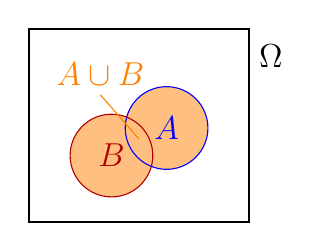
\begin{tikzpicture}[scale=0.7]
\draw[color=black,thick] (-2cm, -1.5cm) rectangle (2cm, 2cm);
\node[color=black,right] at (2cm,1.5cm) {\large{$\Omega$}};
\fill[fill=orange!50] (0.5cm,0.2cm) circle (0.75cm);
\fill[fill=orange!50] (-0.5cm,-0.3cm) circle (0.75cm);
\begin{scope}
\clip (0.5cm,0.2cm) circle (0.75cm);
\fill[fill=orange!50] (-0.5cm,-0.3cm) circle (0.75cm);
\end{scope}
\draw[color=blue] (0.5cm,0.2cm) circle (0.75cm) node {\large{$A$}};
\draw[color=red!70!black] (-0.5cm,-0.3cm) circle (0.75cm) node {\large{$B$}};
\draw[color=orange] (0,0)--(-0.7cm,0.8cm) node[above] {\large{$A\cup B$}};
%\fill[fill=violet!20] (2.125cm,-1.5cm) rectangle +(0.5cm,0.5cm) node[color=violet,pos=0.5,right=0.25cm] {\large{$P$}};
\end{tikzpicture}
\end{center}
\end{minipage}
\begin{minipage}{9.5cm}
\textbf{Réunion d'événements} : l'événement constitué des issues appartenant à $A$ ou à $B$ est noté $A\cup B$
\end{minipage}
\end{defi}

\begin{ex}{}{intersection_lancer_de}
   Avec l'exemple \ref{exe:lancer_de}, on a $A$:\og obtenir un nombre inférieur à $4$ \fg{}. Soit $B$:\og obtenir un nombre pair\fg{}.

   On a $A\cap B = \{2;~4\}$,\quad $A\cap \overline{B} = \{1;~3\}$,\quad $\overline{A}\cap B = \{6\}$ et \quad $\overline{A}\cap \overline{B} = \{5\}$.

   On a $A\cup B=\{1;~2;~3;~4;~6\}$.

% \begin{minipage}{0.6\linewidth}
  \begin{tabular}{|l|c|c|c|}
    \hline
     & $A$ & $\overline{A}$ & Total\\
    \hline
    $B$ & $\P(A\cap B)=\frac{2}{6}=\frac{1}{3}$ & $\P(\overline{A}\cap B)=\frac{1}{6}$ &$\P(B)=\frac{3}{6}=\frac{1}{2}$\\
    \hline
    $\overline{B}$ & $\P(A\cap \overline{B})=\frac{2}{6}=\frac{1}{3}$ & $\P(\overline{A}\cap \overline{B})=\frac{1}{6}$ & $\P(\overline{B})=\frac{3}{6}=\frac{1}{2}$\\
    \hline
    Total & $\P(A)=\frac{4}{6}=\frac{2}{3}$ & $\P(\overline{A})=\frac{2}{6}=\frac{1}{3}$ & $\P(\Omega)=1$ \\
    \hline
  \end{tabular}
% \end{minipage}
% \begin{minipage}{0.35\linewidth}
% \begin{tikzpicture}[
%     level 1/.style={level distance=6em, sibling distance=10em},
%     level 2/.style={level distance=6em, sibling distance=5em},
%     grow'=right,
%     edge from parent/.style={draw, -latex},
%     every node/.style={font=\small, align=center}
% ]

% \coordinate
%   child {
%     node {$A$}
%     child {
%       node {$B$}
%       edge from parent node[above left] {}
%     }
%     child {
%       node {$\overline{B}$}
%       edge from parent node[below left] {}
%     }
%     edge from parent node[above left] {$\P(A) = \frac{2}{3}$}
%   }
%   child {
%     node {$\overline{A}$}
%     child {
%       node {$B$}
%       edge from parent node[above left] {}
%     }
%     child {
%       node {$\overline{B}$}
%       edge from parent node[below left] {}
%     }
%     edge from parent node[below left] {$\P(\overline{A}) = \frac{1}{3}$}
%   };
% \end{tikzpicture}
% \end{minipage}
\end{ex}


\section{Probabilité conditionnelle}

\begin{defi}{Probabilité conditionnelle}{}
	On appelle \textbf{probabilité conditionnelle} de B sachant A, la probabilité que l'événement B se réalise sachant que l'événement A est réalisé. On la note : $\P_A(B)$.
\end{defi}

   Si on cherche à calculer la probabilité de $B$ sachant $A$, on se place dans la colonne $A$. Les issues favorables sont alors $A\cap B$. L'ensemble des issues possibles est $A$.


\begin{theo}{}{}
   Lorsque $\P(A)\ne 0$,
   \begin{minipage}{0.4\linewidth}
       $$\P_A(B) = \frac{\P(A\cap B)}{\P(A)}$$
   \end{minipage}
   \begin{minipage}{0.4\linewidth}
       \begin{center}
      \begin{tabular}{|l|>{\columncolor[gray]{0.8}}c|c|c|}
      \hline
      & $A$ & $\overline{A}$ & Total\\
      \hline
      $B$ & $\P(A\cap B)$ & $\P(\overline{A}\cap B)$ &$\P(B)$\\
      \hline
      $\overline{B}$ & $\P(A\cap \overline{B})$ & $\P(\overline{A}\cap \overline{B})$ & $\P(\overline{B})$\\
      \hline
      Total & $\P(A)$ & $\P(\overline{A})$ & $\P(\Omega)$ \\
      \hline
    \end{tabular}
  \end{center}
  \end{minipage}

  On a également $\P(A\cap B) = \P_A(B)\times \P(A)$ (même si $\P(A)=0$).
\end{theo}


\begin{ex}{}{}
   On reprend l'exemple \ref{exe:intersection_lancer_de} et on calcule les probabilités.

\begin{minipage}{0.35\linewidth}
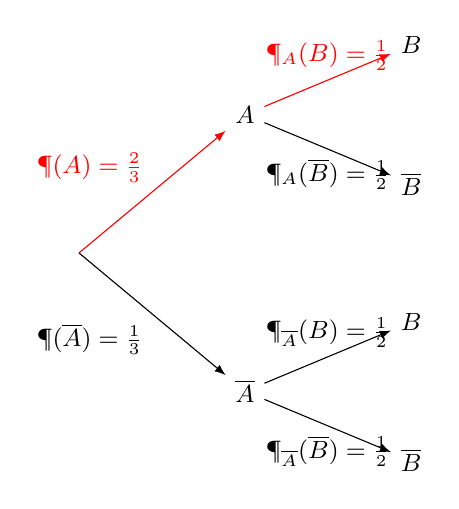
\begin{tikzpicture}[
    level 1/.style={level distance=6em, sibling distance=10em},
    level 2/.style={level distance=6em, sibling distance=5em},
    grow'=right,
    edge from parent/.style={draw, -latex},
    every node/.style={font=\small, align=center}
]

\coordinate
  child {
    node {$A$}
    child {
      node {$B$}
      edge from parent[red] node[above] {$\P_A(B) = \frac{1}{2}$}
    }
    child {
      node {$\overline{B}$}
      edge from parent[black] node[below] {$\P_A(\overline{B})= \frac{1}{2}$}
    }
    edge from parent[red] node[above left] {$\P(A) = \frac{2}{3}$}
  }
  child {
    node {$\overline{A}$}
    child {
      node {$B$}
      edge from parent node[above] {$\P_{\overline{A}}(B)= \frac{1}{2}$}
    }
    child {
      node {$\overline{B}$}
      edge from parent node[below] {$\P_{\overline{A}}(\overline{B})= \frac{1}{2}$}
    }
    edge from parent node[below left] {$\P(\overline{A}) = \frac{1}{3}$}
  };
\end{tikzpicture}
\end{minipage}
\begin{minipage}{0.65\linewidth}
  Une fois les probabilités inscrites sur l'arbre, on peut lire la probabilité des intersections en multipliant les probabilités le long du chemin. Par exemple, $\P(A\cap B) = \P(A)\times \P_A(B)=\frac{2}{3}\times\frac{1}{2}=\frac{1}{3}$.
\end{minipage}
\end{ex}

\begin{rem}{}{}
   Attention à bien faire la différence entre la probabilité $\P(A\cap B)$ que les deux événements se réalisent en même temps et la probabilité $\P_A(B)$ que le second se réalise, sachant que le premier est déjà réalisé.
\end{rem}

\begin{histoire}{}{}
  Le hasard n'a pas toujours été un domaine d'études mathématiques. Pendant toute l'antiquité, le hasard sert à créer des jeux, au divertissement. C'est davantage une question de philosphie. Il faut attendre le XVIIe sièclepour que Huygens donne des définitions précises du concept de probabilités. Dans \textit{The Doctrine of Chances} publié à Londres en 1718, Abraham de Moivre (1667-1754) est le premier mathématicien à aborder la notion d'indépendance d'événements. C'est à une œuvre de Thomas Bayes (1702-1761), publiée à titre posthume, que l'on doit la première théorie sur les probabilités conditionnelles.

  La théorie des probabilités a toujours pris une place à part dans le domaine des mathématiques et beaucoup de mathématiciens ont rejeté cette théorie dans un premier temps. Joseph Bertrand en 1900 écrit : « Comment oser parler des lois du hasard ? Le hasard n'est-il pas l'antithèse de toute loi ? ».
\end{histoire}

\section{Indépendance d'événements}
\begin{defi}{Evénements Indépendants}{}
    Lorsque la réalisation d'un événement $B$ ne dépend pas de la réalisation de l'événement $A$, on dit qu'ils sont indépendants. Mathématiquement, on traduit cela par :
    $$\P_A(B) = \P(B)$$
\end{defi}

\begin{ex}{}{}
    Lorsqu'on lance deux dés successivement, chaque lancer est indépendant. Le résultat du premier dé n'a aucune influence sur le résultat du deuxième.

    Dans l'exemple \ref{exe:intersection_lancer_de}, on a calculé $\P_A(B) = \frac{1}{2}$ et $\P(B)=\frac{1}{2}$. Donc les événements $A$ et $B$ sont indépendants.

    On peut aussi le voir en considérant qu'il est aussi probable d'avoir $B$ : \og un numéro pair \fg{} parmi l'ensemble des résultats du dé $\{~1~;~2~;~3~;~4~;~5~;~6~\}$ que parmi les nombres $\{~1~;~2~;~3~;~4~\}$ correspondant à la réalisation de $A$.
\end{ex}

\begin{prop}{Symétrie de l'indépendance}{}
    Soit $A$ et $B$ deux événements de probabilité non nulle. $A$ est indépendant de $B$ si et seulement si $B$ est indépendant de $A$.
\end{prop}

\begin{dem}{}{}
    On suppose que $A$ est indépendant de $B$. Alors $\P_A(B) = \P(B)$ ou encore $\frac{\P(A\cap B)}{\P(A)} = \P(B)$.

    Donc $\P(A\cap B) = \P(A) \times \P(B)$.

    On calcule alors: $\P_B(A) = \frac{\P(A\cap B)}{\P(B)} = \frac{\P(A) \times \P(B)}{\P(B)} = \P(A)$.

    Donc $B$ est indépendant de $A$.
\end{dem}

\section{Probabilités totales}
\begin{defi}{Partition}{}
  On se donne des événements $A_1, A_2, \dots, A_n$. Lorsque chaque issue appartient à un et un seul des événements, on dit qu'ils forment une partition de l'univers en $n$ événements.
\end{defi}

\begin{ex}{}{}
  $A$ et $\overline{A}$ forment une partition car $A\cup \overline{A} = \Omega$. On a couvert toutes les issues possibles une et une seule fois.

  Soit $A$:\og obtenir un nombre inférieur à $4$ \fg{} et $B$:\og obtenir un nombre supérieur à $4$ \fg{}. Ils ne forment pas une partition de l'univers car ils ne sont pas disjoints. On a $A \cap B = \{4\}$. Autrement dit, $4$ est compté deux fois.
\end{ex}

\begin{theo}{Formule des probabilités totales}{}
  Soit une partition de l'univers en $n$ événements $A_1, A_2, \dots, A_n$. Soit $B$ un autre événement. On a:

  $$\P(B) = \P_{A_1}(B)\times \P(A_1) + \P_{A_2}(B)\times \P(A_2) + \dots + \P_{A_n}(B)\times \P(A_n)$$
\end{theo}

\begin{ex}{}{}
  Pour une partition en deux événements $A$ et $\overline{A}$, la formule devient $\P(B) = \P_{A}(B)\times \P(A) + \P_{\overline{A}}(B)\times \P(\overline{A})$.
\end{ex}

\begin{dem}{}{}
  Démontrons le théorème dans le cas d'une partition de l'univers en deux événements $A_1$ et $A_2$.

  Puisque la partition de l'univers couvre toute les possibilités une et une seule fois, on peut décomposer l'événements $B$ entre les issues qui sont dans $A_1$ et les issues qui sont dans $A_2$. On obtient alors:

  \begin{minipage}{0.45\linewidth}
    $\P(B) = \P(B \cap A_1) + \P(B \cap A_2)$
  \end{minipage}
  \begin{minipage}{0.45\linewidth}
    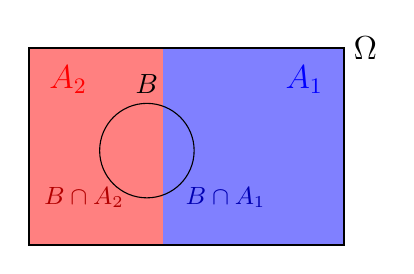
\begin{tikzpicture}
\fill[fill=blue!50] (-0.3, -1.5) rectangle (2, 1);
\node[color=blue] at (1.5,0.6) {\large{$A_1$}};
\fill[fill=red!50] (-2, -1.5) rectangle (-0.3, 1);
\node[color=red] at (-1.5,0.6) {\large{$A_2$}};
\draw[color=black,thick] (-2, -1.5) rectangle (2, 1);
\node[color=black,right] at (2, 1) {\large{$\Omega$}};
\draw (-0.5,-0.3) circle (0.6);
\node[above] at (-0.5, 0.3) {$B$};
\node[red!70!black] at (-1.3, -0.9) {\small{$B\cap A_2$}};
\node[blue!70!black] at (0.5, -0.9) {\small{$B\cap A_1$}};
\end{tikzpicture}
  \end{minipage}

  \vspace{.5cm}
  Avec la définition de probabilité conditionnelle, on remplace:

  $$\P(B) = \P_{A_1}(B)\times \P(A_1) + \P_{A_2}(B)\times \P(A_2)$$

La formule se lit aussi sur l'arbre de probabilités :

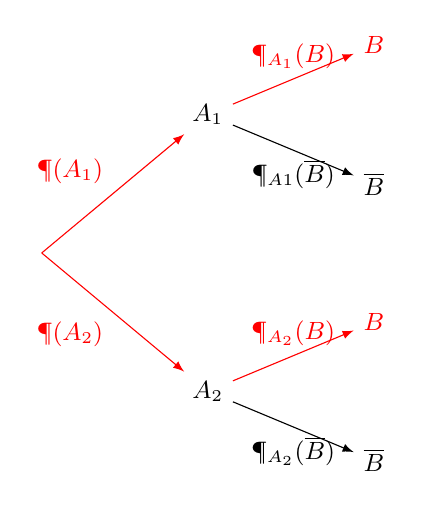
\begin{tikzpicture}[
    level 1/.style={level distance=6em, sibling distance=10em},
    level 2/.style={level distance=6em, sibling distance=5em},
    grow'=right,
    edge from parent/.style={draw, -latex},
    every node/.style={font=\small, align=center}
]

\coordinate
  child {
    node {$A_1$}
    child {
      node[red] {$B$}
      edge from parent[red] node[above] {$\P_{A_1}(B)$}
    }
    child {
      node {$\overline{B}$}
      edge from parent[black] node[below] {$\P_{A1}(\overline{B})$}
    }
    edge from parent[red] node[above left] {$\P(A_1)$}
  }
  child {
    node {$A_2$}
    child {
      node[red] {$B$}
      edge from parent[red] node[above] {$\P_{A_2}(B)$}
    }
    child {
      node {$\overline{B}$}
      edge from parent[black] node[below] {$\P_{A_2}(\overline{B})$}
    }
    edge from parent[red] node[below left] {$\P(A_2)$}
  };
\end{tikzpicture}


\end{dem}



\section*{Exercices}
% \begin{exercices}
	\sectionexo{Vocabulaire probabiliste}
	\begin{bookexos}{15 p.139}\end{bookexos}

  \sectionexo{Intersection d'événement}

  \sectionexo{Probabilité conditionnelle}
  \begin{bookexo}{18 p.139}\end{bookexo}
  \begin{bookact}{1 p.130}\end{bookact}
  \begin{bookact}{2 p.130}\end{bookact}

  \sectionexo{Probabilités totales}
  \begin{bookact}{3 p.134}\end{bookact}
  \begin{bookexo}{37 p.141}\end{bookexo}

  \begin{bookexo}{70 p.145}\end{bookexo}

  \sectionexo{Parcours de révision}
  \begin{bookexo}{85 p.148}\end{bookexo}
  \begin{bookexo}{87 p.149}\end{bookexo}
  \begin{bookexo}{sujet B p.156}\end{bookexo}
  \begin{bookexo}{92 p.149}\end{bookexo}
% \end{exercices}

\end{document}